\documentclass[12pt]{article}

\usepackage{tikz}
\usetikzlibrary{automata}

\usepackage[a4paper,width=150mm,top=25mm,bottom=25mm]{geometry}

\usepackage{amsmath}

\usepackage[T1]{fontenc}

\usepackage{amssymb}

\usepackage{mathtools}
\DeclarePairedDelimiter\floor{\lfloor}{\rfloor}

\usepackage{fancyhdr}
\pagestyle{fancy}
\fancyhead{}
\fancyhead[RO]{Zadania Viktar Zhdanovich}
\fancyfoot{}
\fancyfoot[RO]{\textbf{\thepage}}
\fancyfoot[CO]{Zadania Viktar Zhdanovich}
\renewcommand{\headrulewidth}{0.4pt}
\renewcommand{\footrulewidth}{0.4pt}

\begin{document}

\begin{titlepage}
	\begin{center}
		{\LARGE\bfseries WSTĘP DO TEORII 			OBLICZALNOŚCI\par}
		\vspace{3cm}
		ZADANIA DLA CHĘTNYCH \par
		Zestaw 1. Wersja 1.0.0 \par
	\end{center}
	\vfill\centering VIKTAR ZHDANOVICH LB6 \par
\end{titlepage}

\newpage

\noindent\textbf{Zad 1.1.} Zaprojektuj  maszynę  Turinga,  która  oblicza  funkcję  odejmowania ograniczonego \textit{f} dla liczb naturalnych \textit{m} i \textit{n} w reprezentacji unarnej, czyli
\[ f(m,n) = m - n = 
  \begin{cases}
   	m - n, & \text{jeżeli } m \geq n, \\
   	0, & \text{jezeli } m < n
  \end{cases}
\]
Narysuj diagram przejść. Dla zaprojektowanej maszyny wykonaj dwa obliczenia (wykonaj rysunki taśmy i zapisz konfiguracje).

 Rozwiązanie.
 
\[M=(Q,\Gamma,\Sigma,\delta,q_0,\bigtriangledown,F)=(\{q_0,...,q_7\},\{1,0\},\{1,0,\bigtriangledown\},\delta,q_0,\bigtriangledown,\{q_7\}).\]

\begin{center}
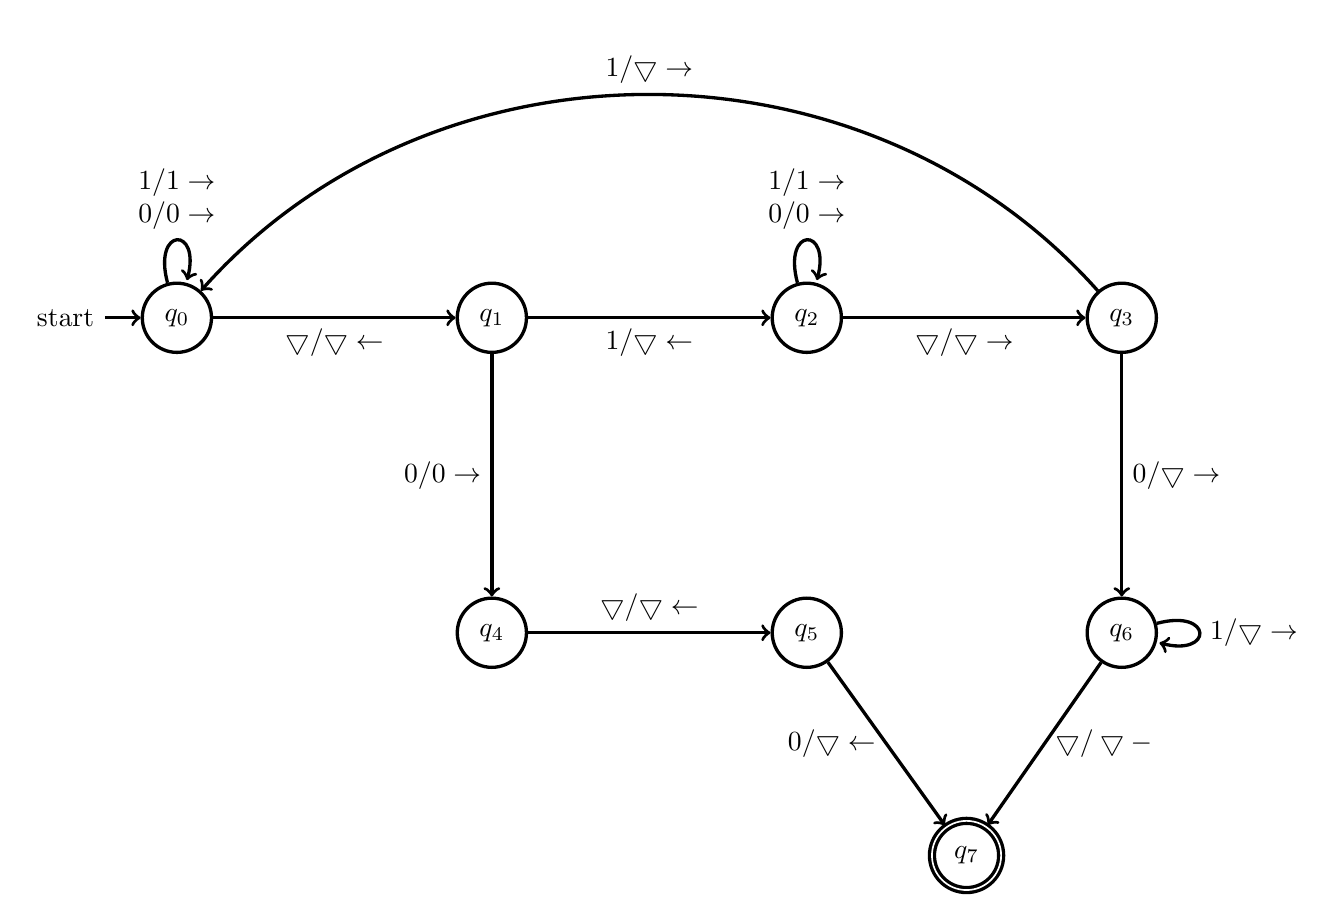
\begin{tikzpicture}[->,node distance=4cm,auto,very thick]

\node[initial,state](q0){$q_0$};
\node[state](q1)[right of=q0]{$q_1$};
\node[state](q4)[below of=q1]{$q_4$};
\node[state](q5)[right of=q4]{$q_5$};
\node[state](q2)[right of=q1]{$q_2$};
\node[state](q3)[right of=q2]{$q_3$};
\node[state](q6)[below of=q3]{$q_6$};
\node[state,accepting](q7)[below right of=q5,xshift=-0.8cm]{$q_7$};

\path(q0)edge node[below]{$\bigtriangledown/\bigtriangledown\leftarrow$}(q1)
	(q0)edge[loop above] node[text 						width=1cm,align=center]{$1/1\rightarrow$\\$0/0\rightarrow$}()
	(q1)edge node[below]{$1/\bigtriangledown\leftarrow$}(q2)
	(q2)edge[loop above] node[text 						width=1cm,align=center]{$1/1\rightarrow$\\$0/0\rightarrow$}()
	(q2)edge node[below]{$\bigtriangledown/\bigtriangledown\rightarrow$}(q3)
	(q3)edge[bend right=1.7cm] node[above]{$1/\bigtriangledown\rightarrow$}(q0)
	(q3)edge node[right]{$0/\bigtriangledown\rightarrow$}(q6)
	(q6)edge[loop right] node[right]{$1/\bigtriangledown\rightarrow$}()
	(q6)edge node[right]{$\bigtriangledown/\bigtriangledown-$}(q7)
	(q1)edge node[left]{$0/0\rightarrow$}(q4)
	(q4)edge node[above]{$\bigtriangledown/\bigtriangledown\leftarrow$}(q5)
	(q5)edge node[left]{$0/\bigtriangledown\leftarrow$}(q7);
	
\end{tikzpicture}
\end{center}

\newpage
\noindent\textbf{Zad 1.2.} Zaprojektuj maszynę Turinga, która oblicza funkcję mnożenia \textit{f} dla liczb naturalnych \textit{m} i \textit{n} w reprezentacji unarnej, czyli
\[f(m,n)=m \cdot n\]
Narysuj diagram przejść. Dla zaprojektowanej maszyny wykonaj dwa obliczenia, w tym pomnóż 3·2 lub 2·3 (wykonaj rysunki taśmy i zapisz konfiguracje).

 Rozwiązanie.
 
\[M=(Q,\Gamma,\Sigma,\delta,q_0,\bigtriangledown,F)=(\{q_0, ... ,q_{11}\},\{1,0\},\{1,0,r,X,Y,\bigtriangledown\},\delta,q_0,\bigtriangledown,\{q_{11}\}).\]

\begin{center}
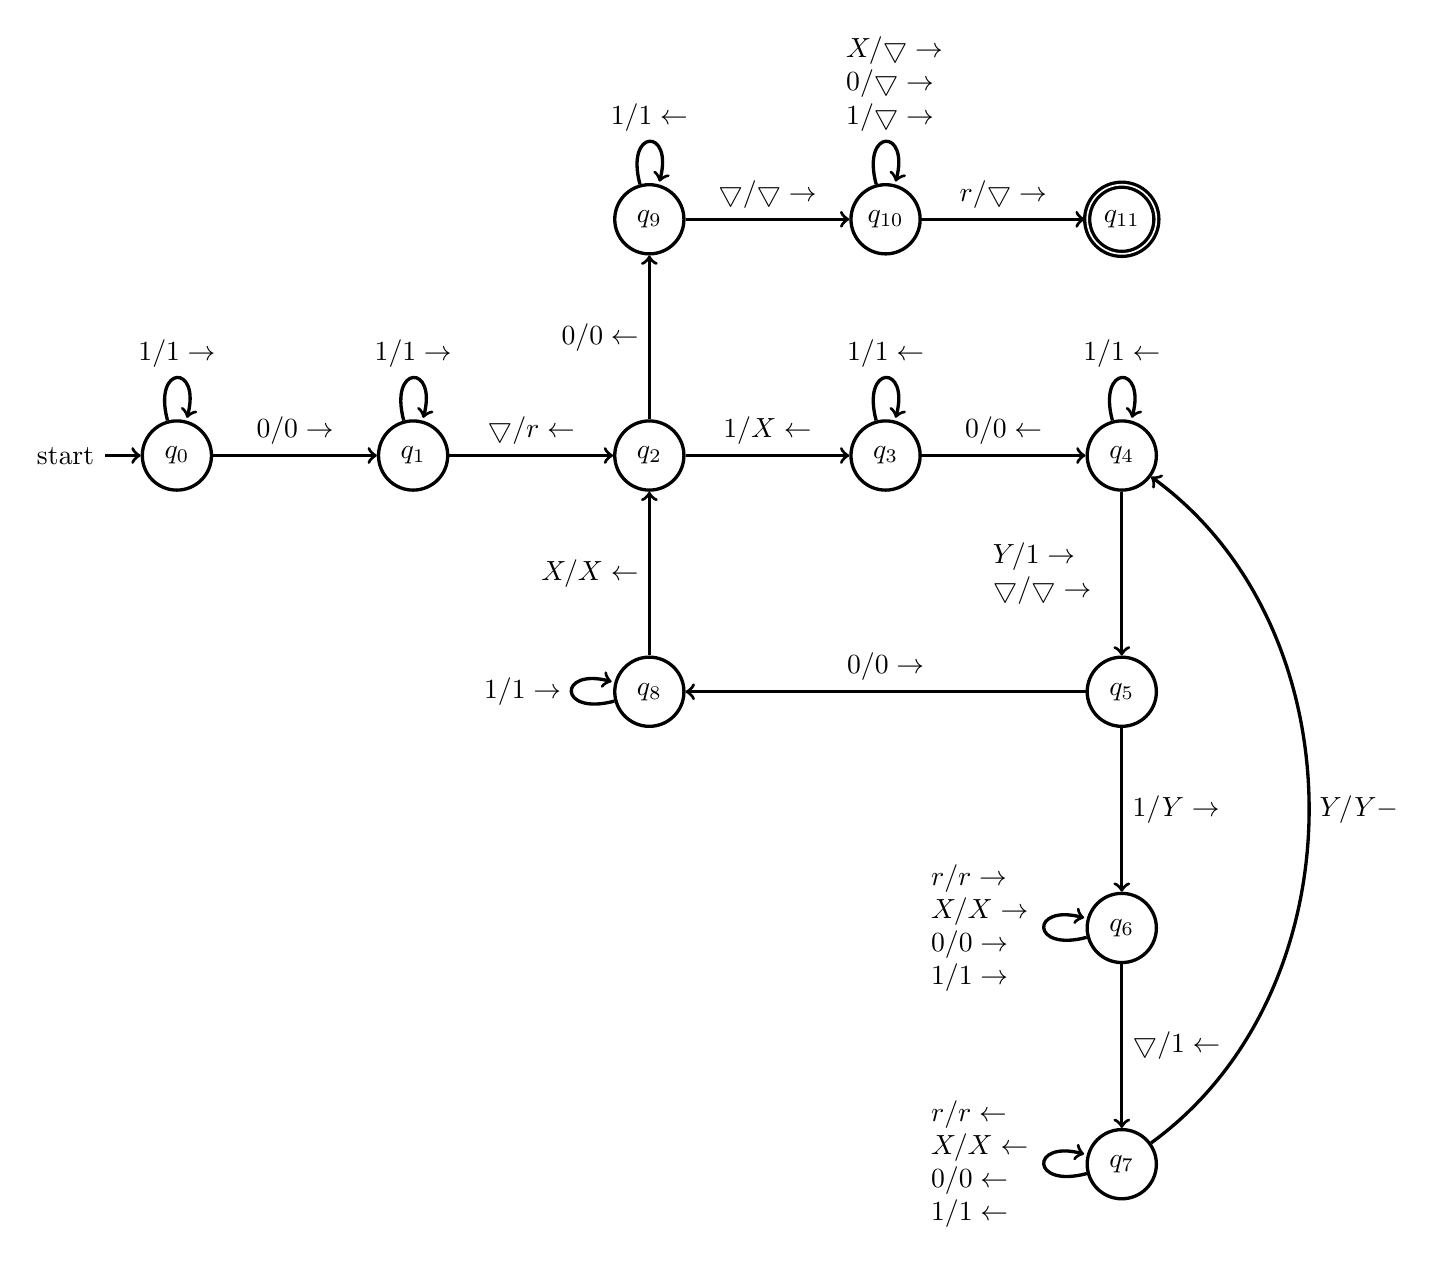
\begin{tikzpicture}[->,node distance=3cm,auto,very thick]

\node[initial,state](q0){$q_0$};
\node[state](q1)[right of=q0]{$q_1$};
\node[state](q2)[right of=q1]{$q_2$};
\node[state](q3)[right of=q2]{$q_3$};
\node[state](q4)[right of=q3]{$q_4$};
\node[state](q5)[below of=q4]{$q_5$};
\node[state](q6)[below of=q5]{$q_6$};
\node[state](q7)[below of=q6]{$q_7$};
\node[state](q8)[below of=q2]{$q_8$};
\node[state](q9)[above of=q2]{$q_9$};
\node[state](q10)[right of=q9]{$q_{10}$};
\node[state,accepting](q11)[right of=q10]{$q_{11}$};

\path(q0)edge node[above]{$0/0\rightarrow$}(q1)
	(q0)edge[loop above] node[above]{$1/1\rightarrow$}()
	(q1)edge node[above]{$\bigtriangledown/r\leftarrow$}(q2)
	(q1)edge[loop above] node[above]{$1/1\rightarrow$}()
	(q2)edge node[above]{$1/X\leftarrow$}(q3)
	(q2)edge node[left]{$0/0\leftarrow$}(q9)
	(q9)edge node[above]{$\bigtriangledown/\bigtriangledown\rightarrow$}(q10)
	(q10)edge node[above]{$r/\bigtriangledown\rightarrow$}(q11)
	(q3)edge node[above]{$0/0\leftarrow$}(q4)
	(q3)edge[loop above] node[above]{$1/1\leftarrow$}()
	(q4)edge[loop above] node[above]{$1/1\leftarrow$}()
	(q4)edge node[text 						width=1cm,left,xshift=-0.5cm]{$Y/1\rightarrow$\\$\bigtriangledown/\bigtriangledown\rightarrow$}(q5)
	(q5)edge node[right]{$1/Y\rightarrow$}(q6)
	(q5)edge node[above]{$0/0\rightarrow$}(q8)
	(q8)edge node[left]{$X/X\leftarrow$}(q2)
	(q6)edge node[right]{$\bigtriangledown/1\leftarrow$}(q7)
	(q7)edge[bend right=1.9cm]node[right]{$Y/Y-$}(q4)
	(q6)edge[loop left] node[text 						width=1cm,left,xshift=-0.3cm]{$r/r\rightarrow$\\$X/X\rightarrow$\\$0/0\rightarrow$\\$1/1\rightarrow$}()
	(q7)edge[loop left] node[text 						width=1cm,left,xshift=-0.3cm]{$r/r\leftarrow$\\$X/X\leftarrow$\\$0/0\leftarrow$\\$1/1\leftarrow$}()
	(q8)edge[loop left] node[left]{$1/1\rightarrow$}()
	(q9)edge[loop above] node[above]{$1/1\leftarrow$}()
	(q10)edge[loop above] node[text 						width=1cm,align=center]{$X/\bigtriangledown\rightarrow$\\$0/\bigtriangledown\rightarrow$\\$1/\bigtriangledown\rightarrow$}();

\end{tikzpicture}
\end{center}

\newpage

\noindent\textbf{Zad 1.3.} Zaprojektuj  maszynę  Turinga,  która  oblicza  funkcję \textit{f} dla  liczbynaturalnej \textit{n} w reprezentacji unarnej, gdzie
\[f(n)=
	\begin{cases}
	\frac{n}{2}, & \text{jeżeli \textit{n} jest parzysta,} \\
   	\frac{n+1}{2}, & \text{jezeli \textit{n} jest niparzysta.}
	\end{cases}	
\]
Narysuj diagram przejść. Dla zaprojektowanej maszyny wykonaj dwa obliczenia (wykonaj rysunki taśmy i zapisz konfiguracje).

 Rozwiązanie.
 
\[M=(Q,\Gamma,\Sigma,\delta,q_0,\bigtriangledown,F)=(\{q_0,...,q_9\},\{1\},\{1,X,\bigtriangledown\},\delta,q_0,\bigtriangledown,\{q_9\}).\]

\begin{center}
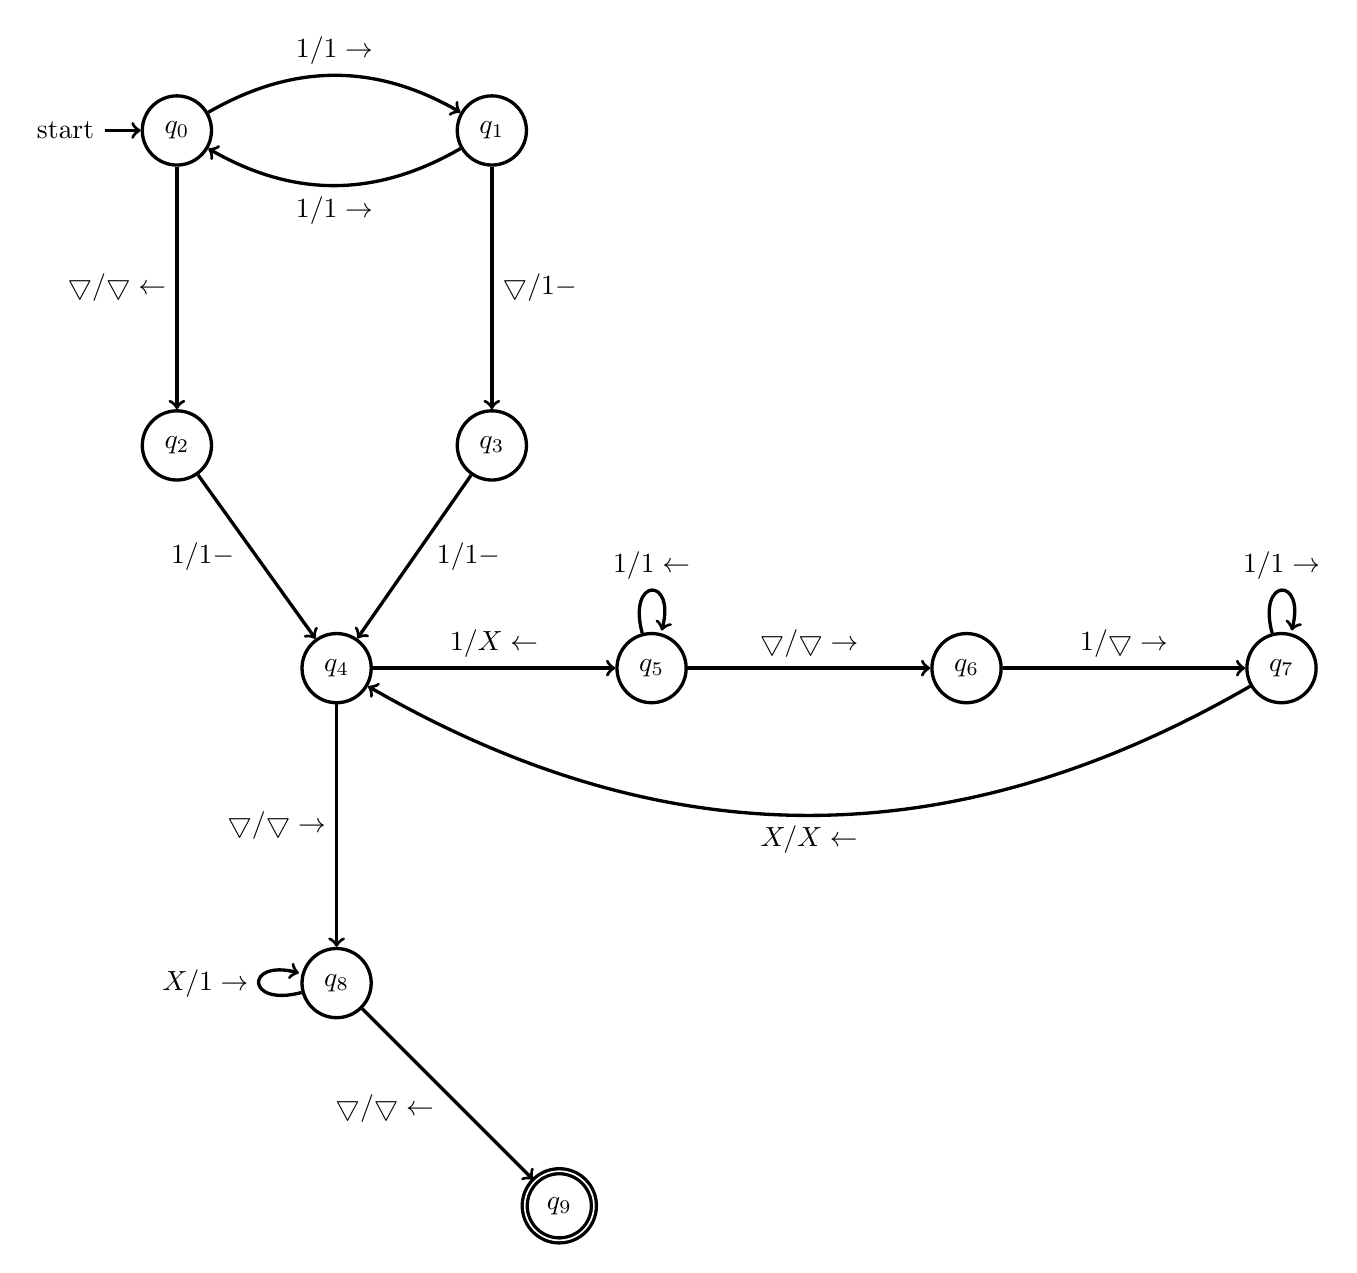
\begin{tikzpicture}[->,node distance=4cm,auto,very thick]

\node[initial,state](q0){$q_0$};
\node[state](q1)[right of=q0]{$q_1$};
\node[state](q2)[below of=q0]{$q_2$};
\node[state](q3)[below of=q1]{$q_3$};
\node[state](q4)[below right of=q2,xshift=-0.8cm]{$q_4$};
\node[state](q5)[right of=q4]{$q_5$};
\node[state](q6)[right of=q5]{$q_6$};
\node[state](q7)[right of=q6]{$q_7$};
\node[state](q8)[below of=q4]{$q_8$};
\node[state,accepting](q9)[below right of=q8]{$q_9$};

\path(q0)edge[bend left] node[above]{$1/1\rightarrow$}(q1)
	 (q1)edge[bend left] node[below]{$1/1\rightarrow$}(q0)
	 (q1)edge node[right]{$\bigtriangledown/1-$}(q3)
	 (q0)edge node[left]{$\bigtriangledown/\bigtriangledown\leftarrow$}(q2)
	 (q3)edge node[right,xshift=0.15cm]{$1/1-$}(q4)
	 (q2)edge node[left,xshift=-0.15cm]{$1/1-$}(q4)
	 (q4)edge node[above]{$1/X\leftarrow$}(q5)
	 (q5)edge[loop above] node[above]{$1/1\leftarrow$}()
	 (q5)edge node[above]{$\bigtriangledown/\bigtriangledown\rightarrow$}(q6)
	 (q6)edge node[above]{$1/\bigtriangledown\rightarrow$}(q7)
	 (q7)edge[loop above] node[above]{$1/1\rightarrow$}()
	 (q7)edge[bend left] node[below]{$X/X\leftarrow$}(q4)
	 (q4)edge node[left]{$\bigtriangledown/\bigtriangledown\rightarrow$}(q8)
	 (q8)edge node[above,xshift=-0.8cm,yshift=-0.5cm]{$\bigtriangledown/\bigtriangledown\leftarrow$}(q9)
	 (q8)edge[loop left] node[left]{$X/1\rightarrow$}();

\end{tikzpicture}
\end{center}

\newpage

\noindent\textbf{Zad 1.5.} Zaprojektuj  maszynę  Turinga,  która  oblicza  funkcję \textit{f} dla  liczby naturalnej \textit{n} w reprezentacji unarnej, gdzie
\[f(n)=\floor*{\frac{n}{2}}\]
Narysuj diagram przejść. Dla zaprojektowanej maszyny wykonaj dwa obliczenia (wykonaj rysunki taśmy i zapisz konfiguracje).

 Rozwiązanie.

\[M=(Q,\Gamma,\Sigma,\delta,q_0,\bigtriangledown,F)=(\{q_0,...,q_6\},\{1\},\{1,X,\bigtriangledown\},\delta,q_0,\bigtriangledown,\{q_6\}).\]

\begin{center}
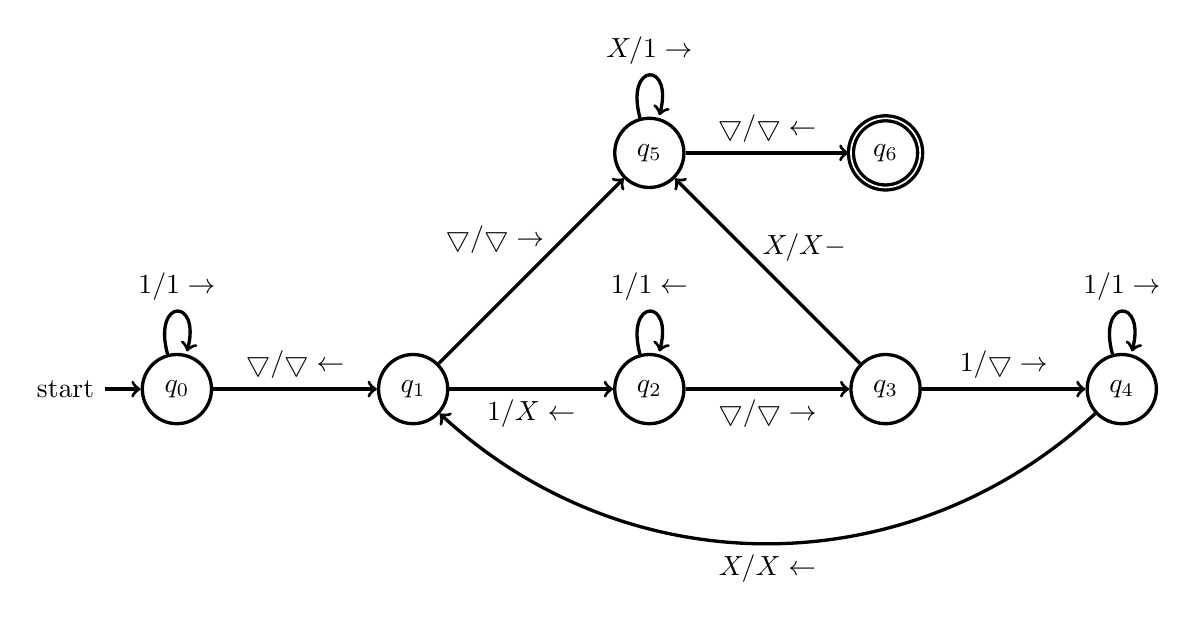
\begin{tikzpicture}[->,node distance=3cm,auto,very thick]

\node[initial,state](q0){$q_0$};
\node[state](q1)[right of=q0]{$q_1$};
\node[state](q2)[right of=q1]{$q_2$};
\node[state](q5)[above of=q2]{$q_5$};
\node[state,accepting](q6)[right of=q5]{$q_6$};
\node[state](q3)[right of=q2]{$q_3$};
\node[state](q4)[right of=q3]{$q_4$};

\path(q0)edge node[above]{$\bigtriangledown/\bigtriangledown\leftarrow$}(q1)
	(q0)edge[loop above] node[above]{$1/1\rightarrow$}()
	(q1)edge node[below]{$1/X\leftarrow$}(q2)
	(q2)edge node[below]{$\bigtriangledown/\bigtriangledown\rightarrow$}(q3) 
	(q2)edge[loop above] node[above]{$1/1\leftarrow$}()
	(q3)edge node[above]{$1/\bigtriangledown\rightarrow$}(q4)
	(q4)edge[bend left=1.5cm] node[below]{$X/X\leftarrow$}(q1)
	(q4)edge[loop above] node[above]{$1/1\rightarrow$}()
	(q1)edge node[left,yshift=0.4cm,xshift=0.3cm]{$\bigtriangledown/\bigtriangledown\rightarrow$}(q5)
	(q3)edge node[right,yshift=0.3cm,xshift=-0.2cm]{$X/X-$}(q5)
	(q5)edge node[above]{$\bigtriangledown/\bigtriangledown\leftarrow$}(q6)
	(q5)edge[loop above] node[above]{$X/1\rightarrow$}();

\end{tikzpicture}
\end{center}

\newpage

\noindent\textbf{Zad 1.7.} Zaprojektuj maszynę Turinga, która oblicza funkcję signum (znaku)
\[sgn(n)=
	\begin{cases}
	1, & \text{jeżeli \textit{n} > 0,} \\
	0, & \text{jeżeli \textit{n} = 0}
	\end{cases}
\]
Narysuj diagram przejść. Dla zaprojektowanej maszyny wykonaj dwa obliczenia (wykonaj rysunki taśmy i zapisz konfiguracje).

 Rozwiązanie.
 
\[M=(Q,\Gamma,\Sigma,\delta,q_0,\bigtriangledown,F)=(\{q_0,q_1,q_2,q_3,q_4\},\{1\},\{1,X,\bigtriangledown\},\delta,q_0,\bigtriangledown,\{q_4\}).\]

\begin{center}
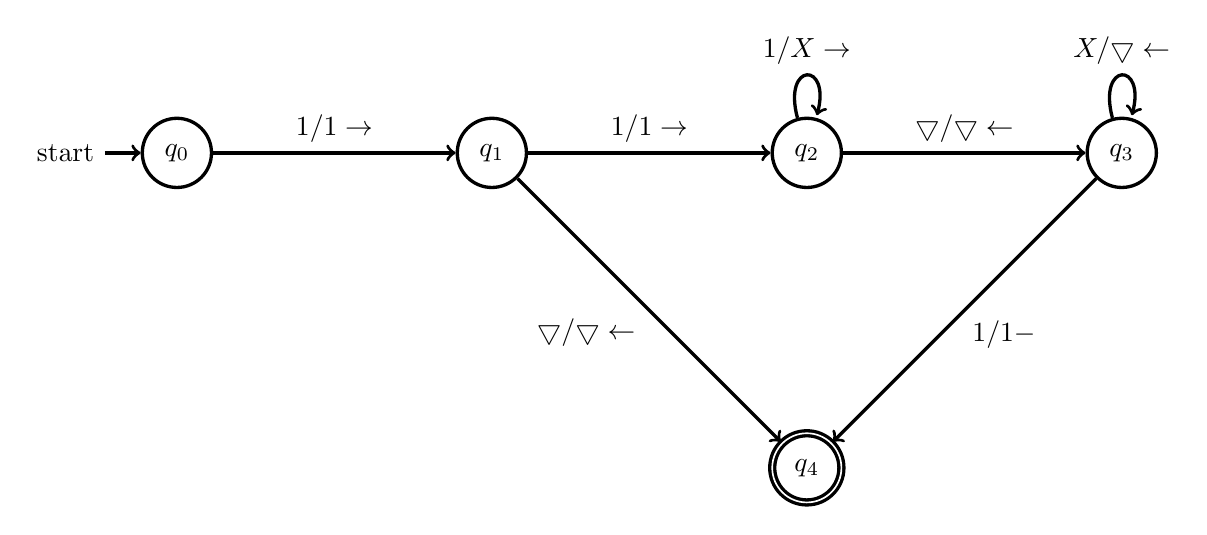
\begin{tikzpicture}[->,node distance=4cm,auto,very thick]

\node[initial,state](q0){$q_0$};
\node[state](q1)[right of=q0]{$q_1$};
\node[state](q2)[right of=q1]{$q_2$};
\node[state](q3)[right of=q2]{$q_3$};
\node[state,accepting](q4)[below of=q2]{$q_4$};

\path(q0)edge node[above]{$1/1\rightarrow$}(q1)
	 (q1)edge node[above]{$1/1\rightarrow$}(q2)
	 (q1)edge node[above,xshift=-0.8cm,yshift=-0.6cm]{$\bigtriangledown/\bigtriangledown\leftarrow$}(q4)
	 (q2)edge node[above]{$\bigtriangledown/\bigtriangledown\leftarrow$}(q3)
	 (q2)edge[loop above] node[above]{$1/X\rightarrow$}()
	 (q3)edge[loop above] node[above]{$X/\bigtriangledown\leftarrow$}()
	 (q3)edge node[below,xshift=0.5cm]{$1/1-$}(q4)
	 ;

\end{tikzpicture}
\end{center}

\newpage

\noindent\textbf{Zad 1.9.} Zaprojektuj maszynę Turinga, która oblicza funkcję
\[f(n)=
	\begin{cases}
	0, & \text{jeżeli \textit{n} jest parzysta,} \\
	1, & \text{jeżeli \textit{n} jest nieparzysta.}
	\end{cases}
\]
Narysuj diagram przejść. Dla zaprojektowanej maszyny wykonaj dwa obliczenia (wykonaj rysunki taśmy i zapisz konfiguracje).

 Rozwiązanie.

\[M=(Q,\Gamma,\Sigma,\delta,q_0,\bigtriangledown,F)=(\{q_0,q_1,q_2,q_3,q_4,q_5\},\{1\},\{1,\bigtriangledown\},\delta,q_0,\bigtriangledown,\{q_5\}).\]

\begin{center}
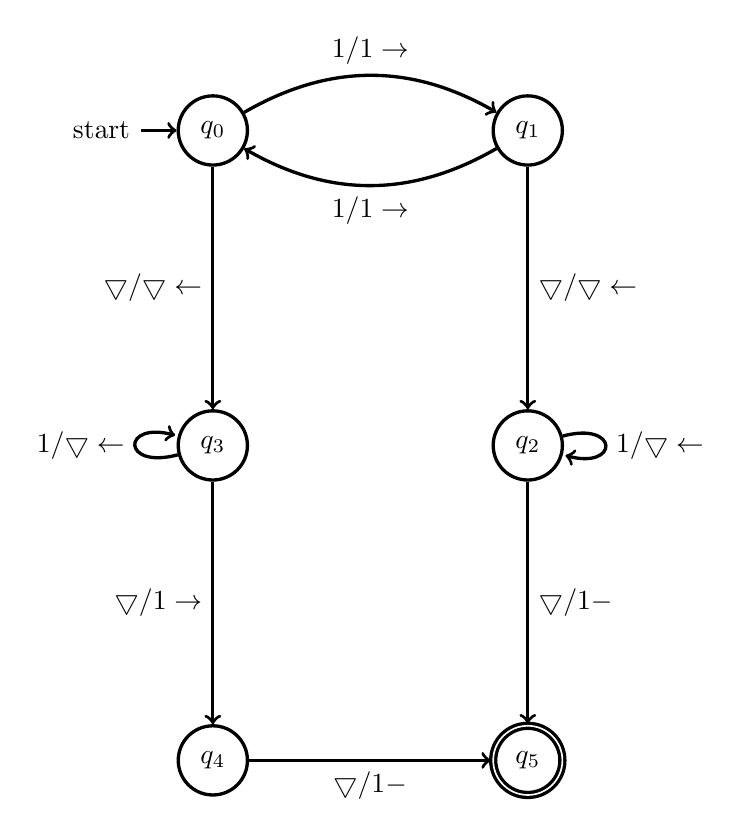
\begin{tikzpicture}[->,node distance=4cm,auto,very thick]

\node[initial,state](q0){$q_0$};
\node[state](q1)[right of=q0]{$q_1$};
\node[state](q2)[below of=q1]{$q_2$};
\node[state](q3)[below of=q0]{$q_3$};
\node[state](q4)[below of=q3]{$q_4$};
\node[state,accepting](q5)[right of=q4]{$q_5$};

\path(q0)edge[bend left] node[above]{$1/1\rightarrow$}(q1)
	(q1)edge[bend left] node[below]{$1/1\rightarrow$}(q0)
	(q1)edge node[right]{$\bigtriangledown/\bigtriangledown\leftarrow$}(q2)
	(q2)edge[loop right] node[right]{$1/\bigtriangledown\leftarrow$}()
	(q2)edge node[right]{$\bigtriangledown/1-$}(q5)
	(q3)edge[loop left] node[left]{$1/\bigtriangledown\leftarrow$}()
	(q0)edge node[left]{$\bigtriangledown/\bigtriangledown\leftarrow$}(q3)
	(q3)edge node[left]{$\bigtriangledown/1\rightarrow$}(q4)
	(q4)edge node[below]{$\bigtriangledown/1-$}(q5);

\end{tikzpicture}
\end{center}

\newpage

\noindent\textbf{Zad 1.11.} Zaprojektuj maszynę Turinga, która oblicza funkcję maksimum dla liczb naturalnych \textit{m} i \textit{n} w reprezentacji unarnej, czyli
\[f(n)=max(m,n).\]
Narysuj diagram przejść. Dla zaprojektowanej maszyny wykonaj dwa obliczenia (wykonaj rysunki taśmy i zapisz konfiguracje).

 Rozwiązanie.
 
\[M=(Q,\Gamma,\Sigma,\delta,q_0,\bigtriangledown,F)=(\{q_0,...,q_{12}\},\{1,0\},\{1,0,X,\bigtriangledown\},\delta,q_0,\bigtriangledown,\{q_{12}\}).\]

\begin{center}
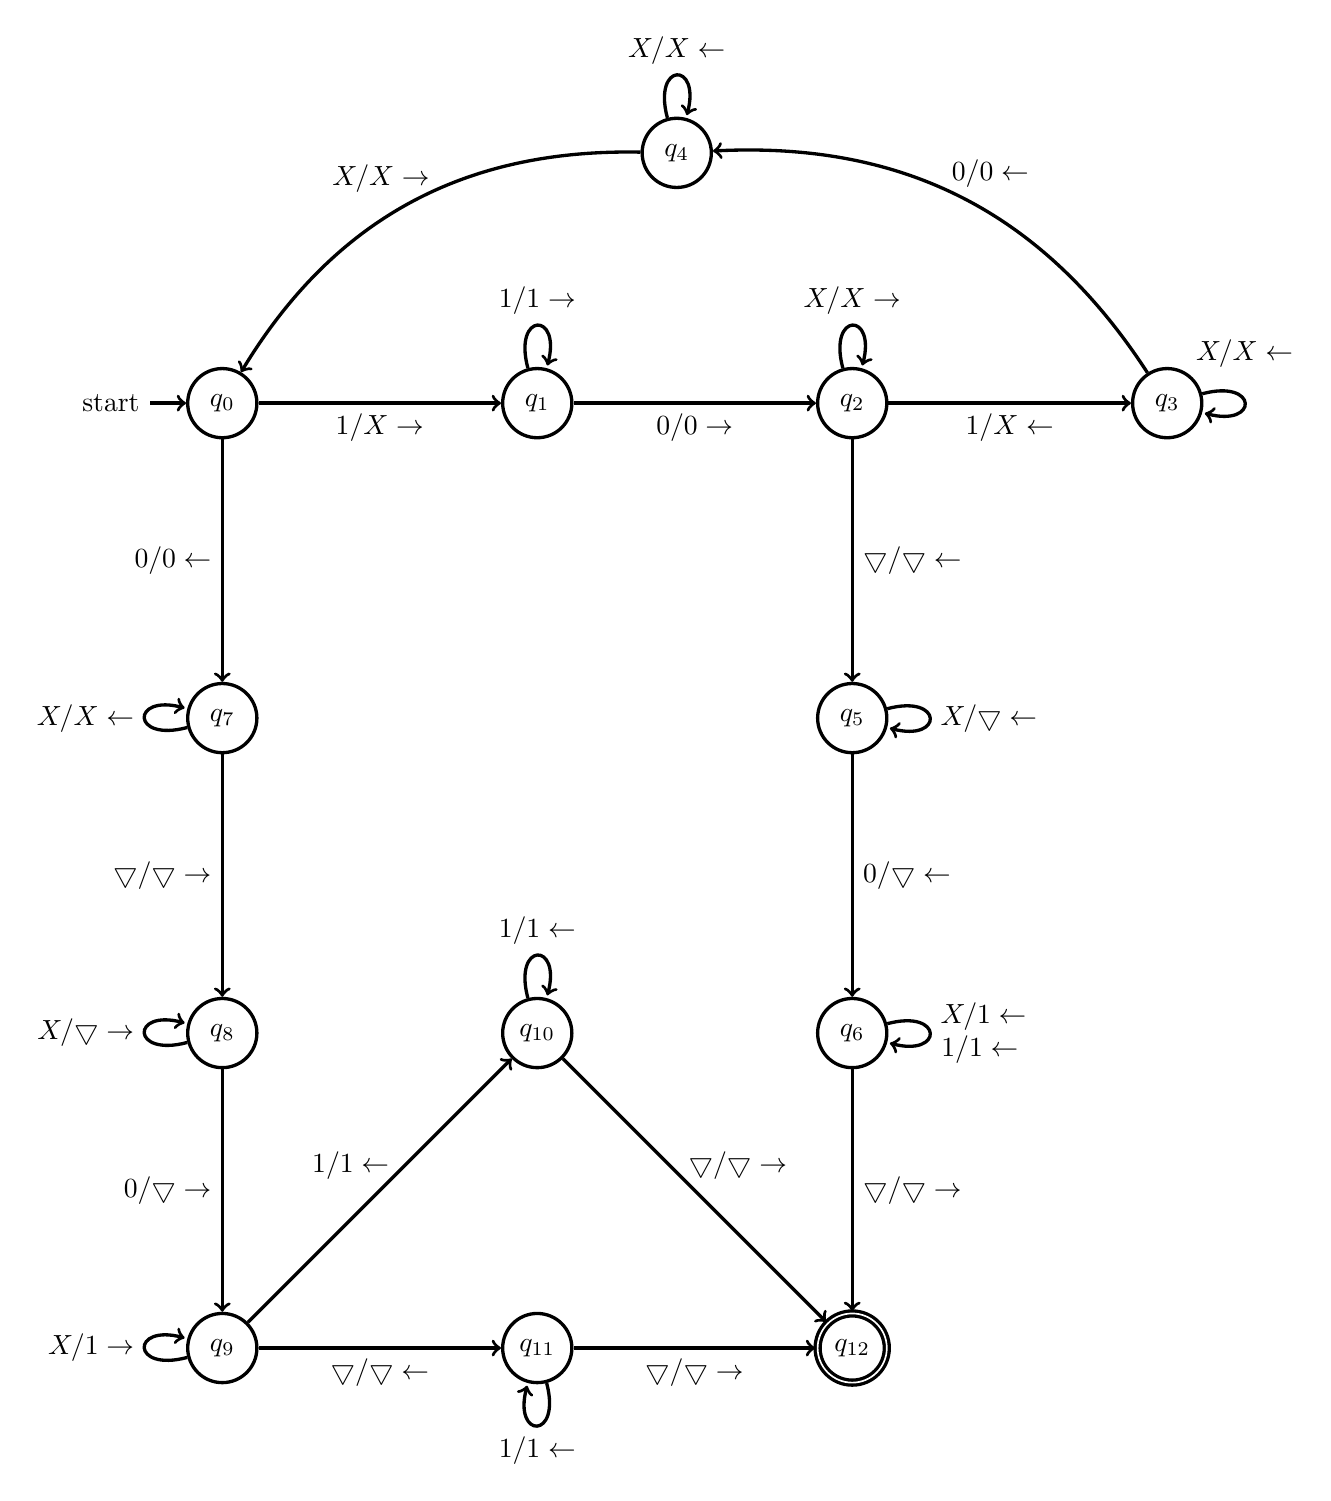
\begin{tikzpicture}[->,node distance=4cm,auto,very thick]

\node[initial,state](q0){$q_0$};
\node[state](q1)[right of=q0]{$q_1$};
\node[state](q2)[right of=q1]{$q_2$};
\node[state](q3)[right of=q2]{$q_3$};
\node[state](q4)[above left of=q2,xshift=0.6cm,yshift=0.35cm]{$q_4$};
\node[state](q5)[below of=q2]{$q_5$};
\node[state](q6)[below of=q5]{$q_6$};
\node[state,accepting](q12)[below of=q6]{$q_{12}$};
\node[state](q7)[below of=q0]{$q_7$};
\node[state](q8)[below of=q7]{$q_8$};
\node[state](q9)[below of=q8]{$q_9$};
\node[state](q11)[right of=q9]{$q_{11}$};
\node[state](q10)[above of=q11]{$q_{10}$};

\path(q0)edge node[below]{$1/X\rightarrow$}(q1)
	(q0)edge node[left]{$0/0\leftarrow$}(q7)
	(q7)edge node[left]{$\bigtriangledown/\bigtriangledown\rightarrow$}(q8)
	(q8)edge node[left]{$0/\bigtriangledown\rightarrow$}(q9)
	(q9)edge node[below]{$\bigtriangledown/\bigtriangledown\leftarrow$}(q11)
	(q9)edge node[above,xshift=-0.37cm]{$1/1\leftarrow$}(q10)
	(q10)edge node[above,xshift=0.55cm]{$\bigtriangledown/\bigtriangledown\rightarrow$}(q12)
	(q11)edge node[below]{$\bigtriangledown/\bigtriangledown\rightarrow$}(q12)
	(q1)edge node[below]{$0/0\rightarrow$}(q2)
	(q1)edge[loop above]node[above]{$1/1\rightarrow$}()
	(q2)edge node[below]{$1/X\leftarrow$}(q3)
	(q2)edge[loop above]node[above]{$X/X\rightarrow$}()
	(q2)edge node[right]{$\bigtriangledown/\bigtriangledown\leftarrow$}(q5)
	(q5)edge node[right]{$0/\bigtriangledown\leftarrow$}(q6)
	(q6)edge node[right]{$\bigtriangledown/\bigtriangledown\rightarrow$}(q12)
	(q3)edge[bend right]node[above,xshift=0.35cm]{$0/0\leftarrow$}(q4)
	(q3)edge[loop right]node[above,yshift=0.32cm]{$X/X\leftarrow$}()
	(q4)edge[bend right]node[above,xshift=-0.35cm]{$X/X\rightarrow$}(q0)
	(q4)edge[loop above]node[above]{$X/X\leftarrow$}()
	(q7)edge[loop left]node[left]{$X/X\leftarrow$}()
	(q8)edge[loop left]node[left]{$X/\bigtriangledown\rightarrow$}()
	(q9)edge[loop left]node[left]{$X/1\rightarrow$}()
	(q5)edge[loop right]node[right]{$X/\bigtriangledown\leftarrow$}()
	(q6)edge[loop right]node[text 						width=1cm,align=center]{$X/1\leftarrow$\\$1/1\leftarrow$}()
	(q10)edge[loop above]node[above]{$1/1\leftarrow$}()
	(q11)edge[loop below]node[below]{$1/1\leftarrow$}();

\end{tikzpicture}
\end{center}

\newpage

\noindent\textbf{Zad 1.13.} Zaprojektuj maszynę Turinga, która oblicza funkcję
\[f(m,n)=n^2\]
dla liczby naturalnej \textit{n} w reprezentacji unarnej. Narysuj diagram przejść. Dla zaprojektowanej maszyny wykonaj dwa obliczenia (wykonaj rysunki taśmy i zapisz konfiguracje).

 Rozwiązanie.
 
\[M=(Q,\Gamma,\Sigma,\delta,q_0,\bigtriangledown,F)=(\{q_0,...,q_{17}\},\{1,0\},\{1,0,X,Y,r,\bigtriangledown\},\delta,q_0,\bigtriangledown,\{q_{11}\}).\]

\begin{center}
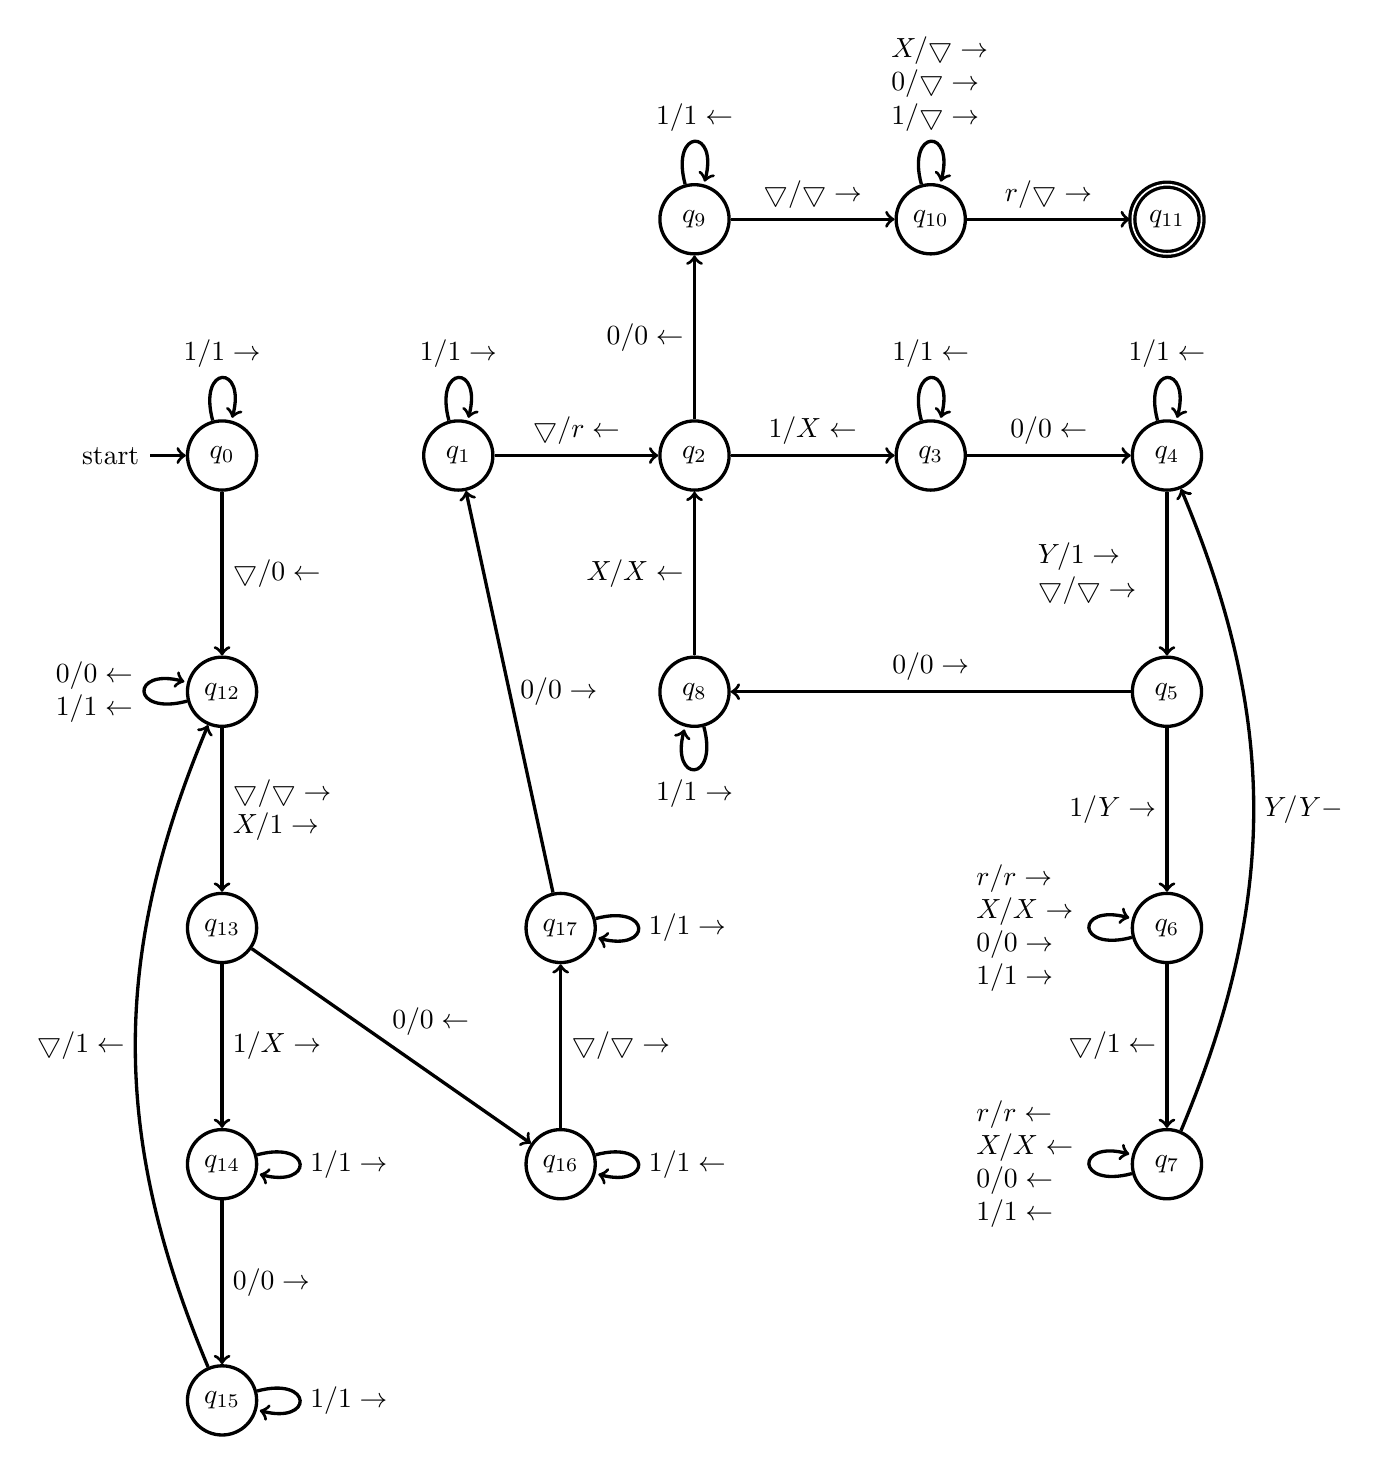
\begin{tikzpicture}[->,node distance=3cm,auto,very thick]

\node[initial,state](q0){$q_0$};
\node[state](q12)[below of=q0]{$q_{12}$};
\node[state](q13)[below of=q12]{$q_{13}$};
\node[state](q14)[below of=q13]{$q_{14}$};
\node[state](q15)[below of=q14]{$q_{15}$};
\node[state](q16)[right of=q14,xshift=1.3cm]{$q_{16}$};
\node[state](q17)[above of=q16]{$q_{17}$};
\node[state](q1)[right of=q0]{$q_1$};
\node[state](q2)[right of=q1]{$q_2$};
\node[state](q3)[right of=q2]{$q_3$};
\node[state](q4)[right of=q3]{$q_4$};
\node[state](q5)[below of=q4]{$q_5$};
\node[state](q6)[below of=q5]{$q_6$};
\node[state](q7)[below of=q6]{$q_7$};
\node[state](q8)[below of=q2]{$q_8$};
\node[state](q9)[above of=q2]{$q_9$};
\node[state](q10)[right of=q9]{$q_{10}$};
\node[state,accepting](q11)[right of=q10]{$q_{11}$};

\path(q0)edge[loop above] node[above]{$1/1\rightarrow$}()
	(q1)edge node[above]{$\bigtriangledown/r\leftarrow$}(q2)
	(q1)edge[loop above] node[above]{$1/1\rightarrow$}()
	(q2)edge node[above]{$1/X\leftarrow$}(q3)
	(q2)edge node[left]{$0/0\leftarrow$}(q9)
	(q9)edge node[above]{$\bigtriangledown/\bigtriangledown\rightarrow$}(q10)
	(q10)edge node[above]{$r/\bigtriangledown\rightarrow$}(q11)
	(q3)edge node[above]{$0/0\leftarrow$}(q4)
	(q3)edge[loop above] node[above]{$1/1\leftarrow$}()
	(q4)edge[loop above] node[above]{$1/1\leftarrow$}()
	(q4)edge node[text 						width=1cm,left,xshift=-0.5cm]{$Y/1\rightarrow$\\$\bigtriangledown/\bigtriangledown\rightarrow$}(q5)
	(q5)edge node[left]{$1/Y\rightarrow$}(q6)
	(q5)edge node[above]{$0/0\rightarrow$}(q8)
	(q8)edge node[left]{$X/X\leftarrow$}(q2)
	(q6)edge node[left]{$\bigtriangledown/1\leftarrow$}(q7)
	(q7)edge[bend right=0.8cm]node[right]{$Y/Y-$}(q4)
	(q6)edge[loop left] node[text 						width=1cm,left,xshift=-0.3cm]{$r/r\rightarrow$\\$X/X\rightarrow$\\$0/0\rightarrow$\\$1/1\rightarrow$}()
	(q7)edge[loop left] node[text 						width=1cm,left,xshift=-0.3cm]{$r/r\leftarrow$\\$X/X\leftarrow$\\$0/0\leftarrow$\\$1/1\leftarrow$}()
	(q8)edge[loop below] node[below]{$1/1\rightarrow$}()
	(q9)edge[loop above] node[above]{$1/1\leftarrow$}()
	(q10)edge[loop above] node[text 						width=1cm,align=center]{$X/\bigtriangledown\rightarrow$\\$0/\bigtriangledown\rightarrow$\\$1/\bigtriangledown\rightarrow$}()
	(q0)edge node[right]{$\bigtriangledown/0\leftarrow$}(q12)
	(q12)edge node[text 						width=1cm,align=center]{$\bigtriangledown/\bigtriangledown\rightarrow$\\$X/1\rightarrow$}(q13)
	(q12)edge[loop left] node[text 						width=1cm,align=center]{$0/0\leftarrow$\\$1/1\leftarrow$}()
	(q13)edge node[right]{$1/X\rightarrow$}(q14)
	(q14)edge node[right]{$0/0\rightarrow$}(q15)
	(q14)edge[loop right] node[right]{$1/1\rightarrow$}()
	(q15)edge[loop right] node[right]{$1/1\rightarrow$}()
	(q16)edge[loop right] node[right]{$1/1\leftarrow$}()
	(q17)edge[loop right] node[right]{$1/1\rightarrow$}()
	(q15)edge[bend left=0.8cm] node[left]{$\bigtriangledown/1\leftarrow$}(q12)
	(q13)edge node[above,xshift=0.5cm]{$0/0\leftarrow$}(q16)
	(q16)edge node[right]{$\bigtriangledown/\bigtriangledown\rightarrow$}(q17)
	(q17)edge node[right]{$0/0\rightarrow$}(q1);

\end{tikzpicture}
\end{center}

\newpage

\noindent\textbf{Zad 1.19.} Zaprojektuj maszynę Turinga, która kopiuje wejściowy łańcuch \textit{w} dla alfabetu $\Sigma=\{a,b\}$. Rozwiązanie może nie zawierać separatora
\[q_0w \overset{*}{\vdash} q_fww\]
lub  może  zawierać  dowolny  separator,  na  przykład  separatorem  może  być blank, czyli
\[q_0w \overset{*}{\vdash} q_fw \bigtriangledown w.\]
Narysuj diagram przejść. Dla zaprojektowanej maszyny wykonaj dwa obliczenia (wykonaj rysunki taśmy i zapisz konfiguracje).

 Rozwiązanie.
 
\[M=(Q,\Gamma,\Sigma,\delta,q_0,\bigtriangledown,F)=(\{q_0,...,q_{10}\},\{a,b\},\{a,b,s,X,Y,\bigtriangledown\},\delta,q_0,\bigtriangledown,\{q_{10}\}).\]

\begin{center}
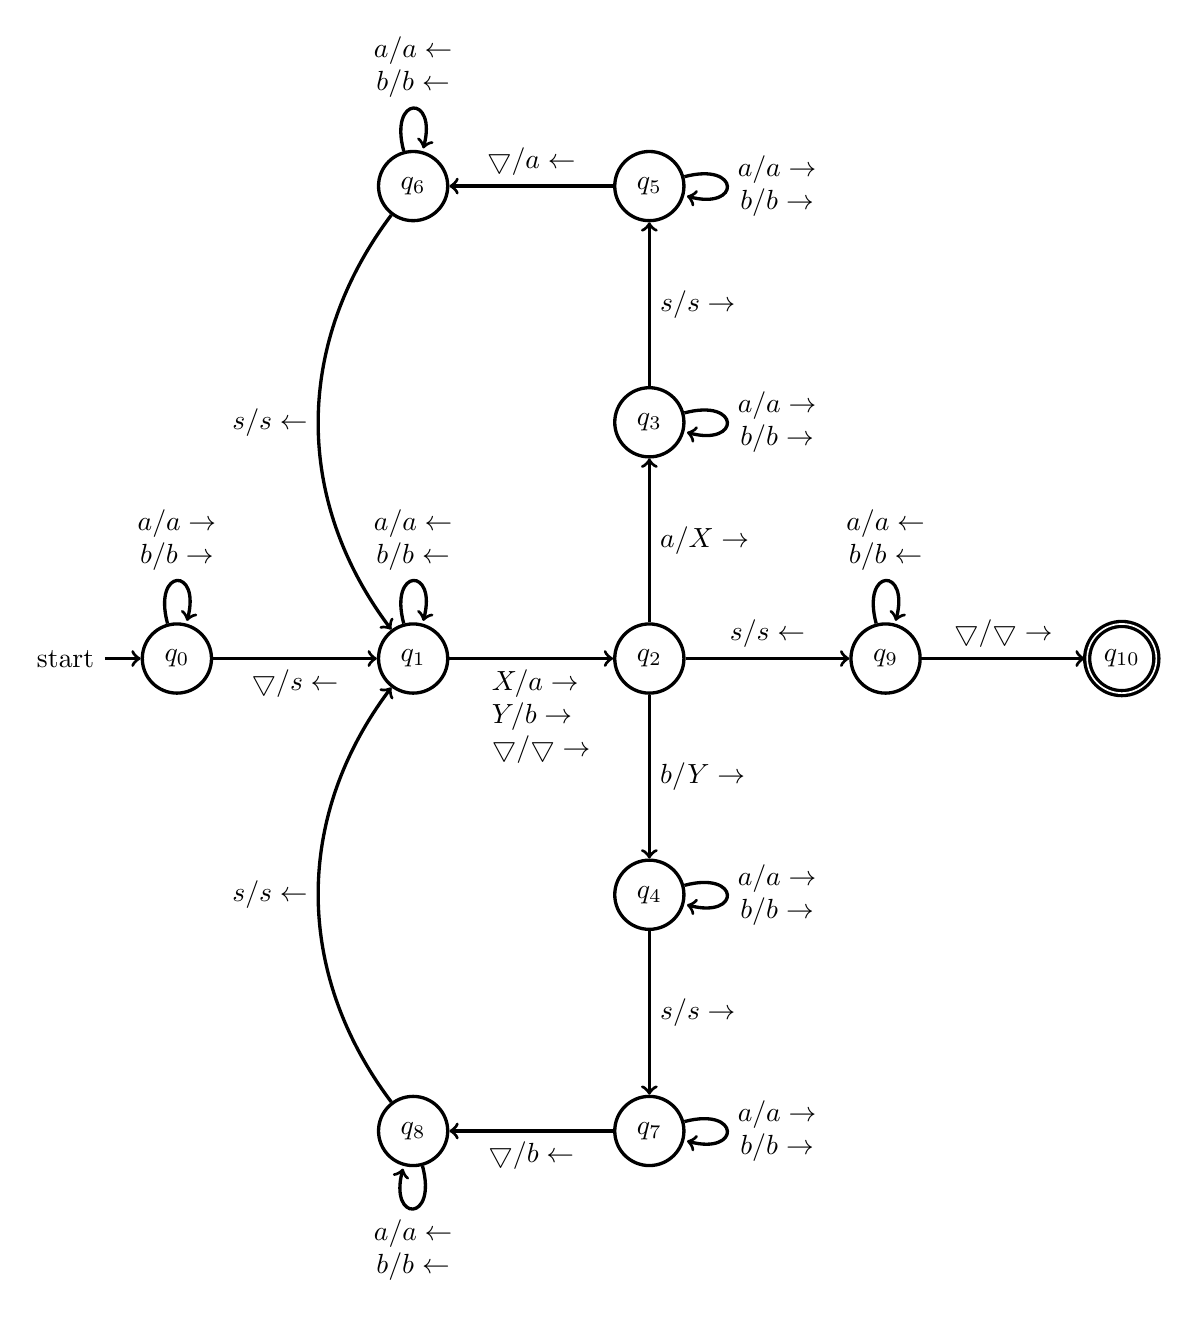
\begin{tikzpicture}[->,node distance=3cm,auto,very thick]

\node[initial,state](q0){$q_0$};
\node[state](q1)[right of=q0]{$q_1$};
\node[state](q2)[right of=q1]{$q_2$};
\node[state](q3)[above of=q2]{$q_3$};
\node[state](q5)[above of=q3]{$q_5$};
\node[state](q6)[left of=q5]{$q_6$};
\node[state](q4)[below of=q2]{$q_4$};
\node[state](q7)[below of=q4]{$q_7$};
\node[state](q8)[left of=q7]{$q_8$};
\node[state](q9)[right of=q2]{$q_9$};
\node[state,accepting](q10)[right of=q9]{$q_{10}$};

\path(q0)edge node[below]{$\bigtriangledown/s\leftarrow$}(q1)
	(q0)edge[loop above] node[text 						width=1cm,align=center]{$a/a\rightarrow$\\$b/b\rightarrow$}()
	(q1)edge node[text 						width=1cm,below,align=center]{$X/a\rightarrow$\\$Y/b\rightarrow$\\$\bigtriangledown/\bigtriangledown\rightarrow$}(q2)
	(q2)edge node[above]{$s/s\leftarrow$}(q9)
	(q2)edge node[right]{$a/X\rightarrow$}(q3)
	(q3)edge node[right]{$s/s\rightarrow$}(q5)
	(q5)edge node[above]{$\bigtriangledown/a\leftarrow$}(q6)
	(q5)edge[loop right] node[text 						width=1cm,align=center]{$a/a\rightarrow$\\$b/b\rightarrow$}()
	(q3)edge[loop right] node[text 						width=1cm,align=center]{$a/a\rightarrow$\\$b/b\rightarrow$}()
	(q4)edge[loop right] node[text 						width=1cm,align=center]{$a/a\rightarrow$\\$b/b\rightarrow$}()
	(q7)edge[loop right] node[text 						width=1cm,align=center]{$a/a\rightarrow$\\$b/b\rightarrow$}()
	(q6)edge[loop above] node[text 						width=1cm,align=center]{$a/a\leftarrow$\\$b/b\leftarrow$}()
	(q8)edge[loop below] node[text 						width=1cm,align=center]{$a/a\leftarrow$\\$b/b\leftarrow$}()
	(q6)edge[bend right=1.3cm] node[left]{$s/s\leftarrow$}(q1)
	(q2)edge node[right]{$b/Y\rightarrow$}(q4)
	(q4)edge node[right]{$s/s\rightarrow$}(q7)
	(q7)edge node[below]{$\bigtriangledown/b\leftarrow$}(q8)
	(q8)edge[bend left=1.3cm] node[left]{$s/s\leftarrow$}(q1)
	(q1)edge[loop above] node[text 						width=1cm,align=center]{$a/a\leftarrow$\\$b/b\leftarrow$}()
	(q9)edge[loop above] node[text 						width=1cm,align=center]{$a/a\leftarrow$\\$b/b\leftarrow$}()
	(q9)edge node[above]{$\bigtriangledown/\bigtriangledown\rightarrow$}(q10);

\end{tikzpicture}
\end{center}

\newpage

\noindent\textbf{Zad 1.22.} Zaprojektuj  maszynę  Turinga  nad  alfabetem $\Sigma=\{a,b\}$,  która akceptuje język
\[L=\{\text{\textit{w}: \textit{w} zawiera  równą liczbę symboli \textit{a} i \textit{b}}\}.\]
Narysuj diagram przejść. Dla zaprojektowanej maszyny wykonaj dwa obliczenia (wykonaj rysunki taśmy i zapisz konfiguracje).

 Rozwiązanie.
 
\[M=(Q,\Gamma,\Sigma,\delta,q_0,\bigtriangledown,F)=(\{q_0,...,q_6\},\{a,b\},\{a,b,X,Y,\bigtriangledown\},\delta,q_0,\bigtriangledown,\{q_6\}).\]

\vspace{20pt}

\begin{center}
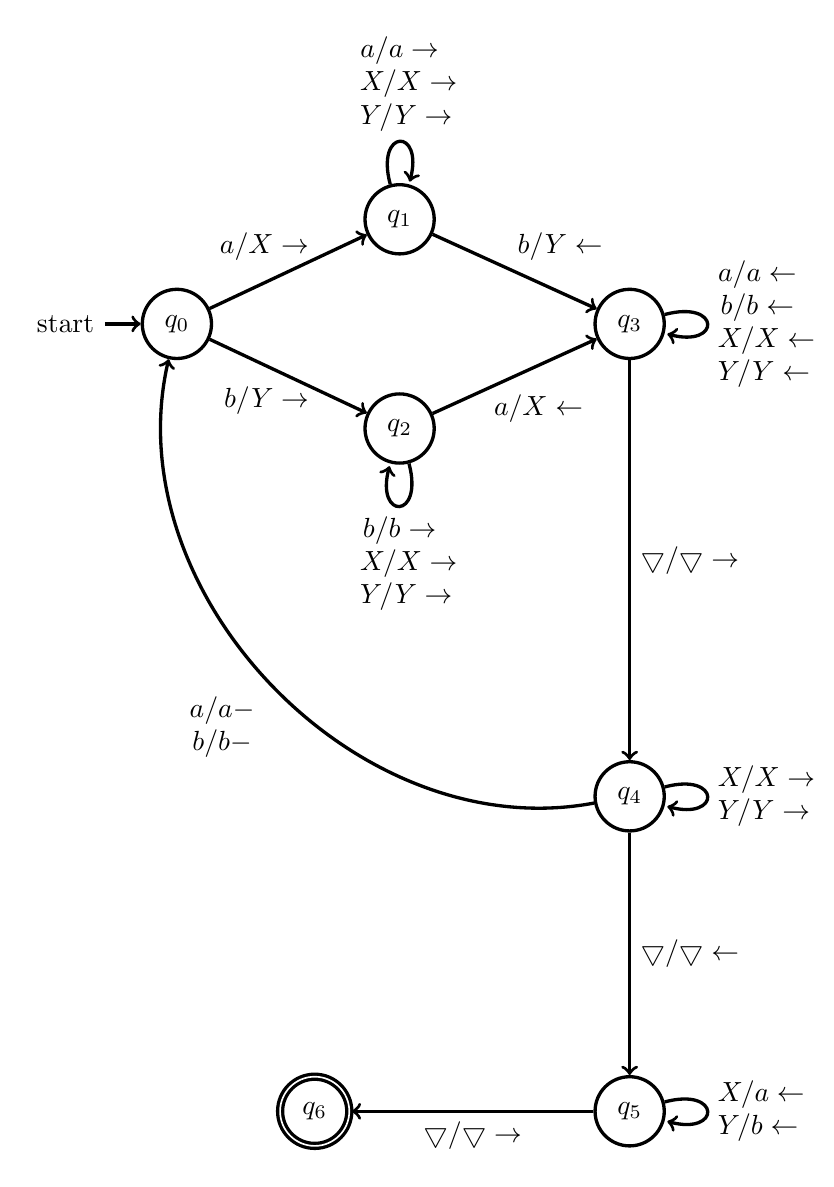
\begin{tikzpicture}[->,node distance=4cm,auto,very thick]

\node[initial,state](q0){$q_0$};
\node[state](q1)[above right of=q0,yshift=-1.5cm]{$q_1$};
\node[state](q2)[below right of=q0,yshift=1.5cm]{$q_2$};
\node[state](q3)[right of=q0,xshift=1.75cm]{$q_3$};
\node[state](q4)[below of=q3,yshift=-2cm]{$q_4$};
\node[state](q5)[below of=q4]{$q_5$};
\node[state,accepting](q6)[left of=q5]{$q_6$};

\path(q0)edge[above right]node[above left,xshift=0.4cm]{$a/X\rightarrow$}(q1)
edge[below right]node[below left,xshift=0.4cm]{$b/Y\rightarrow$}		(q2)
(q2)edge[above right]node[below right,yshift=-0.1cm,xshift=-0.4cm]{$a/X\leftarrow$}(q3)
edge[loop below]node[text 						width=1cm,align=center]{$b/b\rightarrow$\\$X/X\rightarrow$\\$Y/Y\rightarrow$}()
(q1)edge[below right]node[above right,xshift=-0.1cm]{$b/Y\leftarrow$}(q3)
edge[loop above]node[text 						width=1cm,align=center]{$a/a\rightarrow$\\$X/X\rightarrow$\\$Y/Y\rightarrow$}()
(q3)edge[loop right]node[text 						width=1cm,align=center]{$a/a\leftarrow$\\$b/b\leftarrow$\\$X/X\leftarrow$\\$Y/Y\leftarrow$}()
(q3)edge node{$\bigtriangledown/\bigtriangledown\rightarrow$}(q4)
(q4)edge[loop right]node[text 						width=1cm,align=center]{$X/X\rightarrow$\\$Y/Y\rightarrow$}()
edge[bend left=2cm]node[text 						width=1cm,align=center]{$a/a-$\\$b/b-$}(q0)
edge node{$\bigtriangledown/\bigtriangledown\leftarrow$}(q5)
(q5)edge[loop right]node[text 						width=1cm,align=center]{$X/a\leftarrow$\\$Y/b\leftarrow$}()
edge node[below]{$\bigtriangledown/\bigtriangledown\rightarrow$}(q6);

\end{tikzpicture}
\end{center}

\newpage

\noindent\textbf{Zad 1.23.} Zaprojektuj maszynę Turinga, która akceptuje język
\[L=\{\text{\textit{w}: |\textit{w}| jest parzysta}\}\]
nad alfabetem $\Sigma=\{0,1\}$. Narysuj diagram przejść. Dla zaprojektowanej maszyny wykonaj dwa obliczenia (wykonaj rysunki taśmy i zapisz konfiguracje).

 Rozwiązanie.
 
\[M=(Q,\Gamma,\Sigma,\delta,q_0,\bigtriangledown,F)=(\{q_0,q_1,q_2\},\{1,0\},\{1,0,\bigtriangledown\},\delta,q_0,\bigtriangledown,\{q_2\}).\]

\vspace{20pt}

\begin{center}
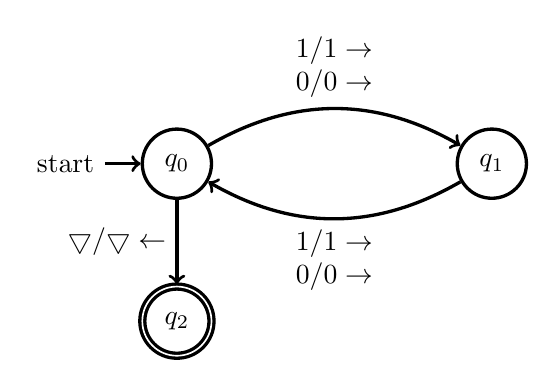
\begin{tikzpicture}[->,node distance=4cm,very thick,auto]

\node[initial,state](q0){$q_0$};
\node[state](q1)[right of=q0]{$q_1$};
\node[state,accepting](q2)[below of=q0,yshift=2cm]{$q_2$};

\path(q0)edge[bend left]node[text 						width=1cm,align=center]{$1/1\rightarrow$\\$0/0\rightarrow$}(q1)
(q0)edge node[left]{$\bigtriangledown/\bigtriangledown\leftarrow$}(q2)
(q1)edge[bend left]node[below,text 						width=1cm,align=center]{$1/1\rightarrow$\\$0/0\rightarrow$}(q0);

\end{tikzpicture}
\end{center}

\newpage

\noindent\textbf{Zad 1.25.} Niech $\Sigma=\{a,b\}$. Zaprojektuj maszynę Turinga, która akceptuje język
\[L=\{\text{\textit{w}${\textit{w}^\textit{R}}$: \textit{w} $\in$ $\{a,b\}^*$\},}\]
gdzie ${\textit{w}^\textit{R}}$ oznacza \textbf{odwrócenie} \textit{w},  a  więc  jeśli \textit{w} = $a_1a_2...a_k$, to ${\textit{w}^\textit{R}}$ = $a_ka_{k-1}...a_1$. Narysuj  diagram  przejść. Dla  zaprojektowanej  maszyny  wykonaj dwa obliczenia (wykonaj rysunki taśmy i zapisz konfiguracje).

 Rozwiązanie.
 
\[M=(Q,\Gamma,\Sigma,\delta,q_0,\bigtriangledown,F)=(\{q_0,...,q_7\},\{a,b\},\{a,b,X,Y,\bigtriangledown\},\delta,q_0,\bigtriangledown,\{q_7\}).\]

\begin{center}
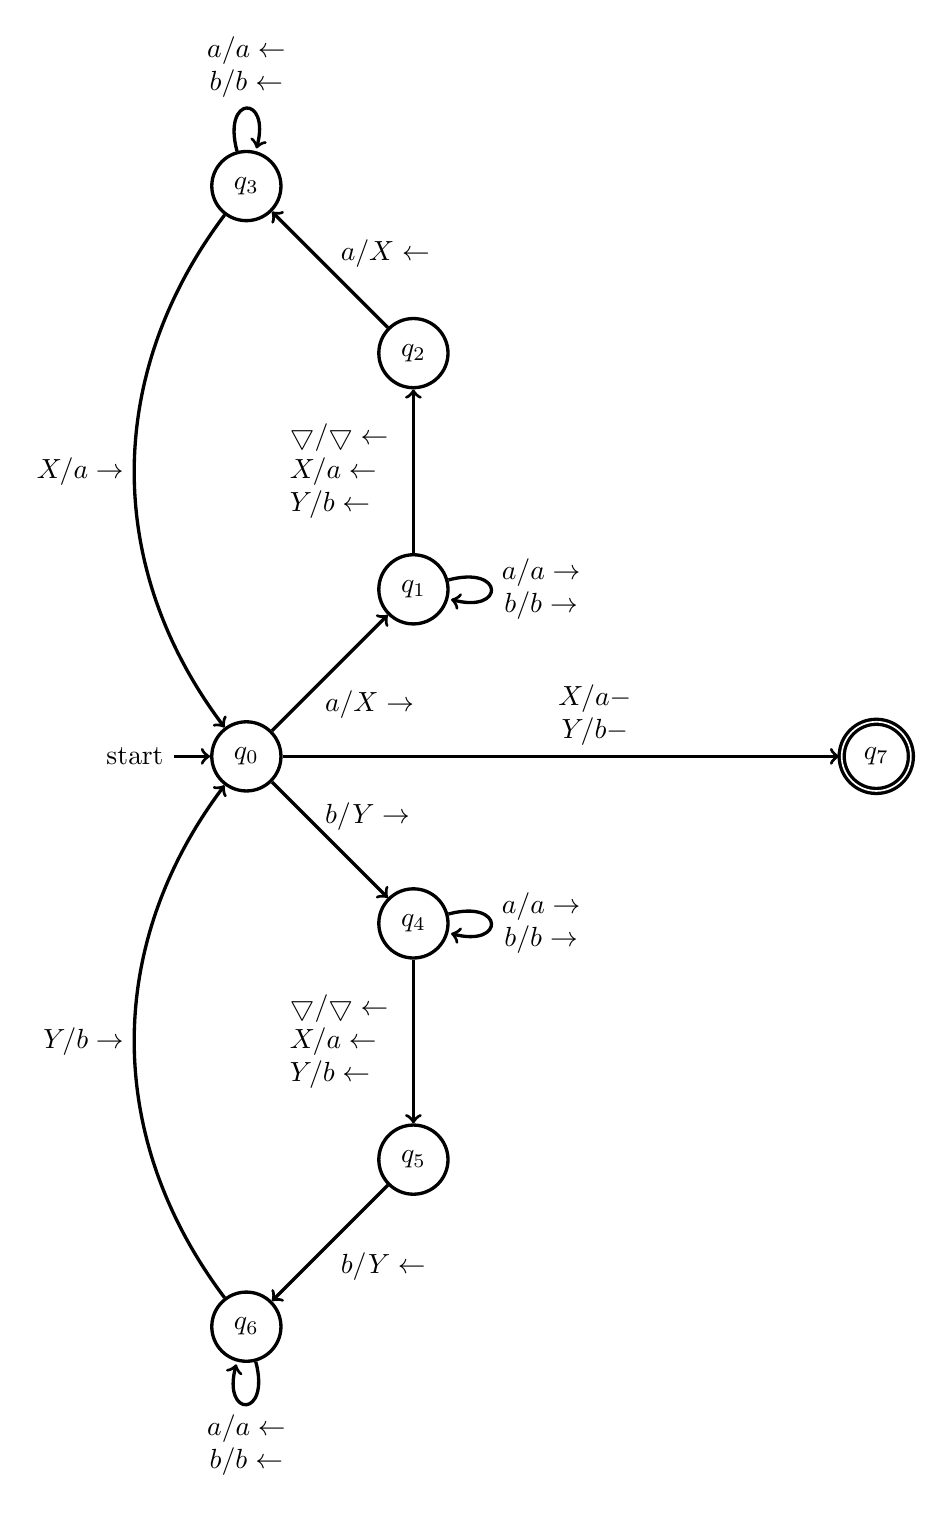
\begin{tikzpicture}[->,node distance=3cm,auto,very thick]

\node[initial,state](q0){$q_0$};
\node[state](q1)[above right of=q0]{$q_1$};
\node[state](q2)[above of=q1]{$q_2$};
\node[state](q3)[above left of=q2]{$q_3$};
\node[state](q4)[below right of=q0]{$q_4$};
\node[state](q5)[below of=q4]{$q_5$};
\node[state](q6)[below left of=q5]{$q_6$};
\node[state,accepting](q7)[right of=q0,xshift=5cm]{$q_7$};

\path(q0)edge node[right,xshift=-0.2cm,yshift=-0.4cm]{$a/X\rightarrow$}(q1)
	(q0)edge node[right,xshift=-0.2cm,yshift=0.3cm]{$b/Y\rightarrow$}(q4)
	(q1)edge node[text 						width=1cm,left,align=center, xshift=-0.43cm]{$\bigtriangledown/\bigtriangledown\leftarrow$\\$X/a\leftarrow$\\$Y/b\leftarrow$}(q2)
	(q2)edge node[right,yshift=0.2cm]{$a/X\leftarrow$}(q3)
	(q4)edge node[text 						width=1cm,left,align=center, xshift=-0.43cm]{$\bigtriangledown/\bigtriangledown\leftarrow$\\$X/a\leftarrow$\\$Y/b\leftarrow$}(q5)
	(q5)edge node[right,yshift=-0.3cm]{$b/Y\leftarrow$}(q6)
	(q0)edge node[text 						width=1cm,above,align=center,xshift=0.43cm]{$X/a-$\\$Y/b-$}(q7)
	(q1)edge[loop right] node[text 						width=1cm,align=center]{$a/a\rightarrow$\\$b/b\rightarrow$}()
	(q3)edge[loop above] node[text 						width=1cm,align=center]{$a/a\leftarrow$\\$b/b\leftarrow$}()
	(q4)edge[loop right] node[text 						width=1cm,align=center]{$a/a\rightarrow$\\$b/b\rightarrow$}()
	(q6)edge[loop below] node[text 						width=1cm,align=center]{$a/a\leftarrow$\\$b/b\leftarrow$}()
	(q3)edge[bend right=1.3cm] node[left]{$X/a\rightarrow$}(q0)
	(q6)edge[bend left=1.3cm] node[left]{$Y/b\rightarrow$}(q0);

\end{tikzpicture}
\end{center}

\newpage

\noindent\textbf{Zad 1.27.} Niech $\Sigma=\{0,1\}$.  Zaprojektuj  maszynę  Turinga,  która  oblicza odwrócenie łańcucha, czyli funkcję
\[f(w)=w^R\]
gdzie $\textit{w}\in\{0,1\}^+$ oraz ${\textit{w}^\textit{R}}$ oznacza \textbf{odwrócenie} \textit{w},  a  więc  jeśli \textit{w} = $a_1a_2...a_k$, to ${\textit{w}^\textit{R}}$ = $a_ka_{k-1}...a_1$. Narysuj  diagram  przejść. Dla  zaprojektowanej  maszyny  wykonaj dwa obliczenia (wykonaj rysunki taśmy i zapisz konfiguracje).

 Rozwiązanie.
 
\[M=(Q,\Gamma,\Sigma,\delta,q_0,\bigtriangledown,F)=(\{q_0,...,q_9\},\{1,0\},\{1,0,s,X,Y,\bigtriangledown\},\delta,q_0,\bigtriangledown,\{q_9\}).\]

\begin{center}
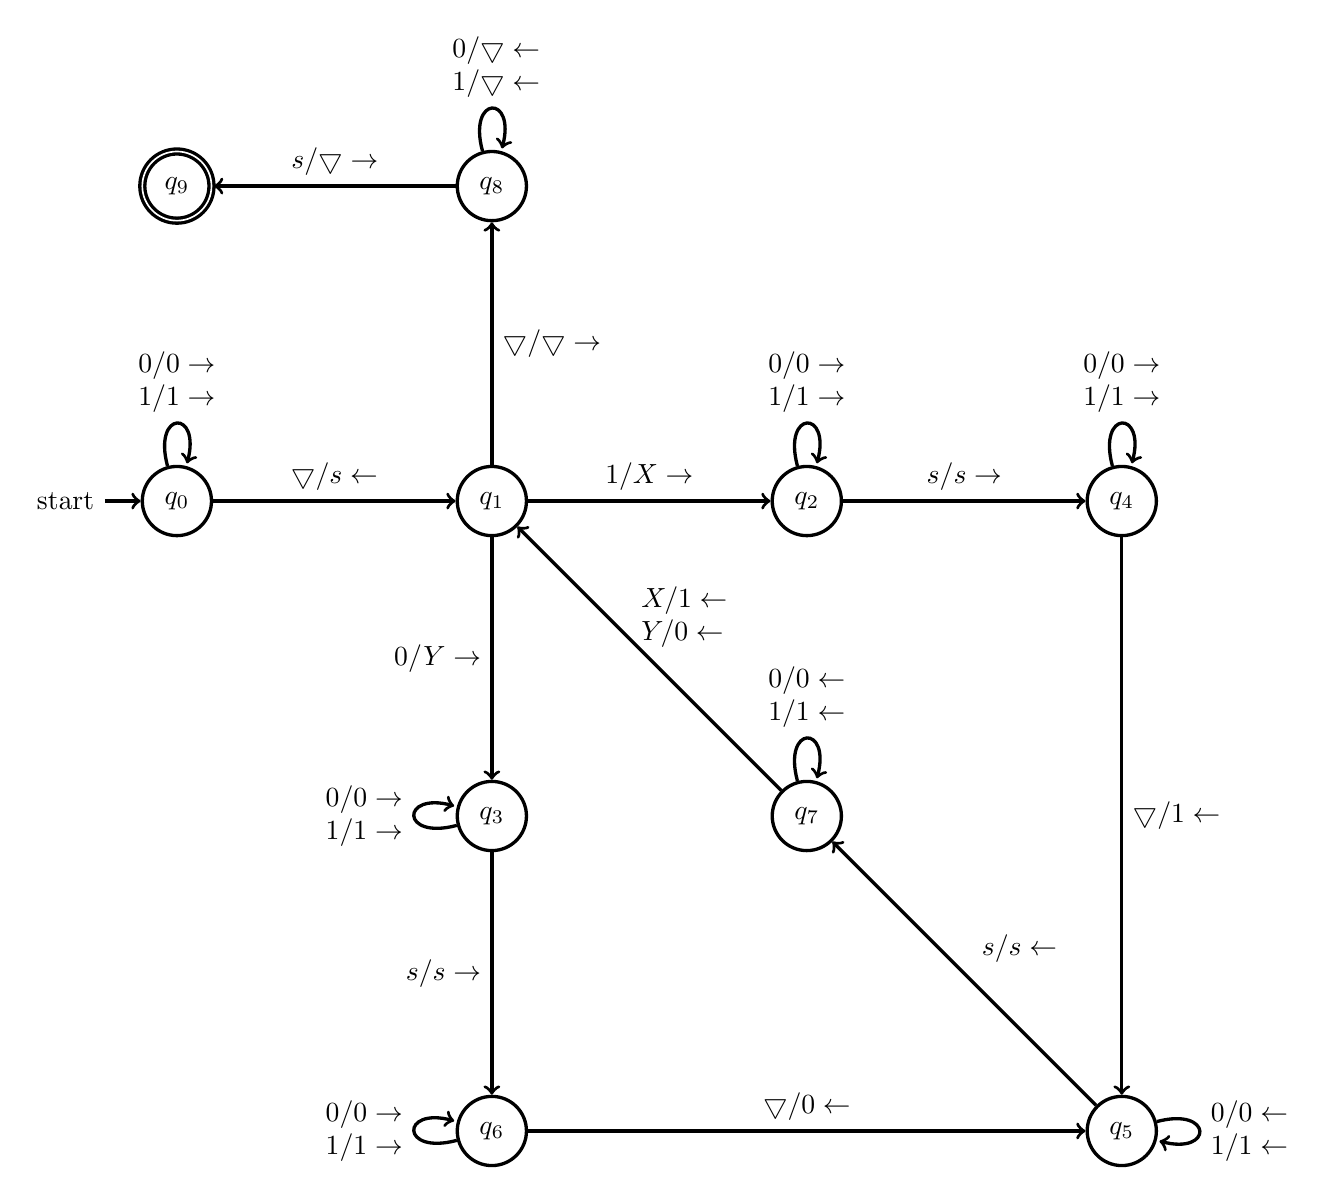
\begin{tikzpicture}[->,node distance=4cm,auto,very thick]

\node[initial,state](q0){$q_0$};
\node[state](q1)[right of=q0]{$q_1$};
\node[state](q2)[right of=q1]{$q_2$};
\node[state](q4)[right of=q2]{$q_4$};
\node[state](q3)[below of=q1]{$q_3$};
\node[state](q6)[below of=q3]{$q_6$};
\node[state](q7)[right of=q3]{$q_7$};
\node[state](q5)[right of=q6,xshift=4cm]{$q_5$};
\node[state](q8)[above of=q1]{$q_8$};
\node[state,accepting](q9)[left of=q8]{$q_9$};

\path(q0)edge node[above]{$\bigtriangledown/s\leftarrow$}(q1)
	(q0)edge[loop above] node[text 						width=1cm,align=center]{$0/0\rightarrow$\\$1/1\rightarrow$}()
	(q1)edge node[left]{$0/Y\rightarrow$}(q3)
	(q1)edge node[above]{$1/X\rightarrow$}(q2)
	(q2)edge node[above]{$s/s\rightarrow$}(q4)
	(q4)edge node[right]{$\bigtriangledown/1\leftarrow$}(q5)
	(q2)edge[loop above] node[text 						width=1cm,align=center]{$0/0\rightarrow$\\$1/1\rightarrow$}()
	(q4)edge[loop above] node[text 						width=1cm,align=center]{$0/0\rightarrow$\\$1/1\rightarrow$}()
	(q3)edge[loop left] node[text 						width=1cm,align=center]{$0/0\rightarrow$\\$1/1\rightarrow$}()
	(q6)edge[loop left] node[text 						width=1cm,align=center]{$0/0\rightarrow$\\$1/1\rightarrow$}()
	(q3)edge node[left]{$s/s\rightarrow$}(q6)
	(q6)edge node[above]{$\bigtriangledown/0\leftarrow$}(q5)
	(q5)edge node[above, xshift=0.7cm]{$s/s\leftarrow$}(q7)
	(q7)edge node[text 						width=1cm,above,xshift=0.4cm,align=center]{$X/1\leftarrow$\\$Y/0\leftarrow$}(q1)
	(q7)edge[loop above] node[text 						width=1cm,align=center]{$0/0\leftarrow$\\$1/1\leftarrow$}()
	(q5)edge[loop right] node[text 						width=1cm,align=center]{$0/0\leftarrow$\\$1/1\leftarrow$}()
	(q1)edge node[right]{$\bigtriangledown/\bigtriangledown\rightarrow$}(q8)
	(q8)edge[loop above] node[text 						width=1cm,align=center]{$0/\bigtriangledown\leftarrow$\\$1/\bigtriangledown\leftarrow$}()
	(q8)edge node[above]{$s/\bigtriangledown\rightarrow$}(q9);

\end{tikzpicture}
\end{center}

\newpage

\noindent\textbf{Zad 1.30.} Zaprojektuj maszynę Turinga, która akceptuje język
\[L=\{\text{$x^ny^n$: \textit{n} $\geq$ 1}\}\]
nad alfabetem $\Sigma=\{x,y\}$. Narysuj diagram przejść. Dla zaprojektowanej maszyny wykonaj dwa obliczenia (wykonaj rysunki taśmy i zapisz konfiguracje).

 Rozwiązanie.
 
\[M=(Q,\Gamma,\Sigma,\delta,q_0,\bigtriangledown,F)=(\{q_0,...,q_8\},\{x,y\},\{x,y,A,B,\bigtriangledown\},\delta,q_0,\bigtriangledown,\{q_8\}).\]

\begin{center}
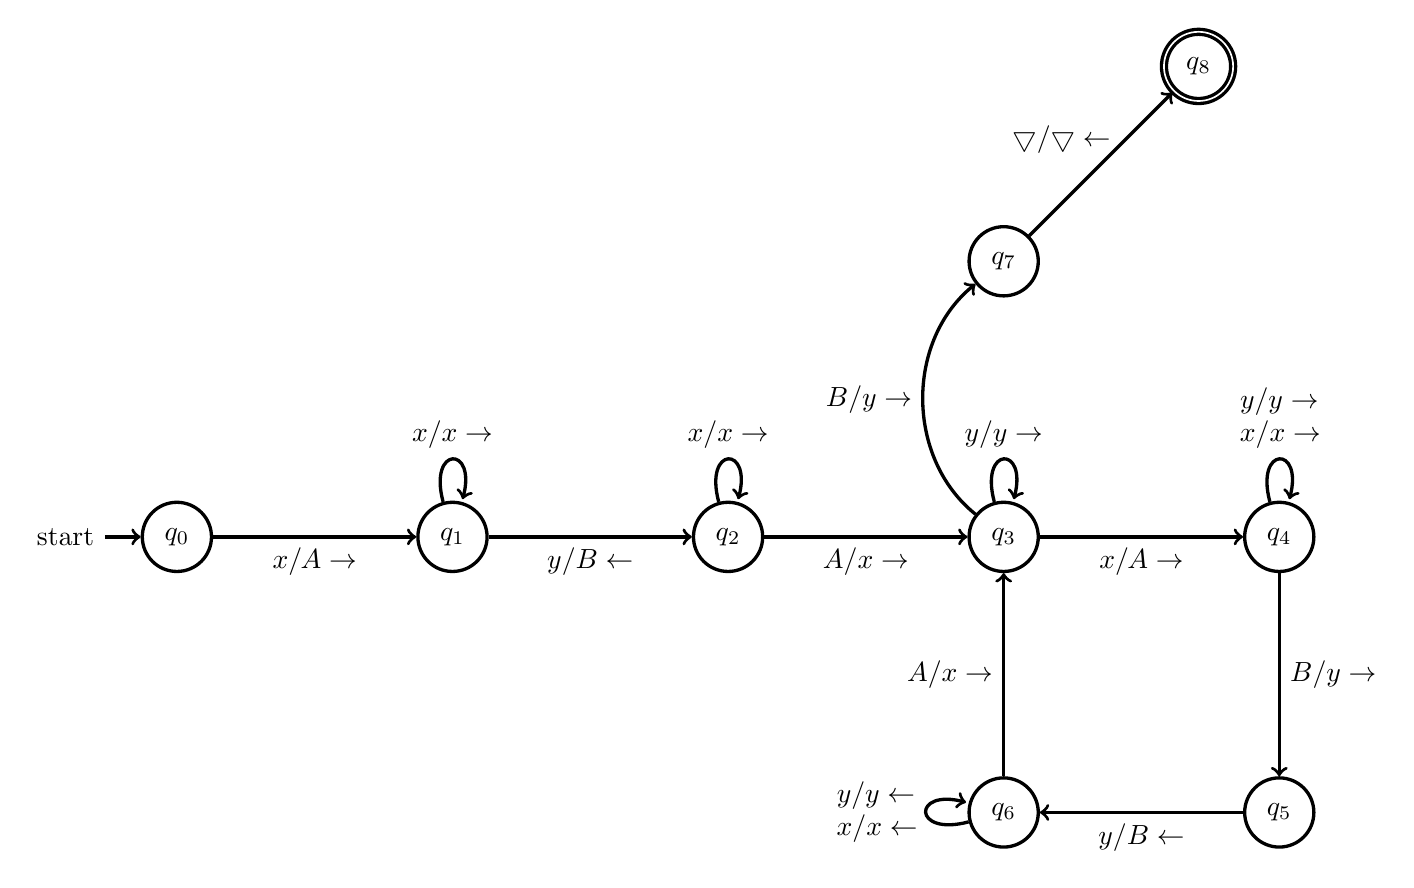
\begin{tikzpicture}[->,node distance=3.5cm,auto,very thick]

\node[initial,state](q0){$q_0$};
\node[state](q1)[right of=q0]{$q_1$};
\node[state](q2)[right of=q1]{$q_2$};
\node[state](q3)[right of=q2]{$q_3$};
\node[state](q4)[right of=q3]{$q_4$};
\node[state](q5)[below of=q4]{$q_5$};
\node[state](q6)[left of=q5]{$q_6$};
\node[state](q7)[above of=q3]{$q_7$};
\node[state,accepting](q8)[above right of=q7]{$q_8$};

\path(q0)edge node[below]{$x/A\rightarrow$}(q1)
	(q1)edge node[below]{$y/B\leftarrow$}(q2)
	(q2)edge node[below]{$A/x\rightarrow$}(q3)
	(q3)edge node[below]{$x/A\rightarrow$}(q4)
	(q4)edge node[right]{$B/y\rightarrow$}(q5)
	(q5)edge node[below]{$y/B\leftarrow$}(q6)
	(q6)edge node[left]{$A/x\rightarrow$}(q3)
	(q3)edge[bend left=1.8cm] node{$B/y\rightarrow$}(q7)
	(q7)edge node[above, xshift=-0.5cm]{$\bigtriangledown/\bigtriangledown\leftarrow$}(q8)
	(q1)edge[loop above] node[above]{$x/x\rightarrow$}()
	(q2)edge[loop above] node[above]{$x/x\rightarrow$}()
	(q3)edge[loop above] node[above]{$y/y\rightarrow$}()
	(q4)edge[loop above] node[text 						width=1cm,align=center]{$y/y\rightarrow$\\$x/x\rightarrow$}()
	(q6)edge[loop left] node[text 						width=1cm,align=center]{$y/y\leftarrow$\\$x/x\leftarrow$}();

\end{tikzpicture}
\end{center}

\newpage

\noindent\textbf{Zad 1.46.} Wypisz cztery przykładowe łańcuchy opisywane przez wyrażenie \textbf{a}$(\textbf{a}+\textbf{b})^*$\textbf{bb}. Czy można skonstruować (deterministyczną) maszynę Turinga,która akceptuje język
\[L=L(\textbf{a}(\textbf{a}+\textbf{b})^*\textbf{bb})?\]
Jeżeli można, to narysuj diagram przejść i dla zaprojektowanej maszyny wykonaj dwa obliczenia (wykonaj rysunki taśmy i zapisz konfiguracje).

 Rozwiązanie.
 
\[M=(Q,\Gamma,\Sigma,\delta,q_0,\bigtriangledown,F)=(\{q_0,q_1,q_2,q_3,q_4\},\{a,b\},\{a,b,\bigtriangledown\},\delta,q_0,\bigtriangledown,\{q_4\}).\]

\begin{center}
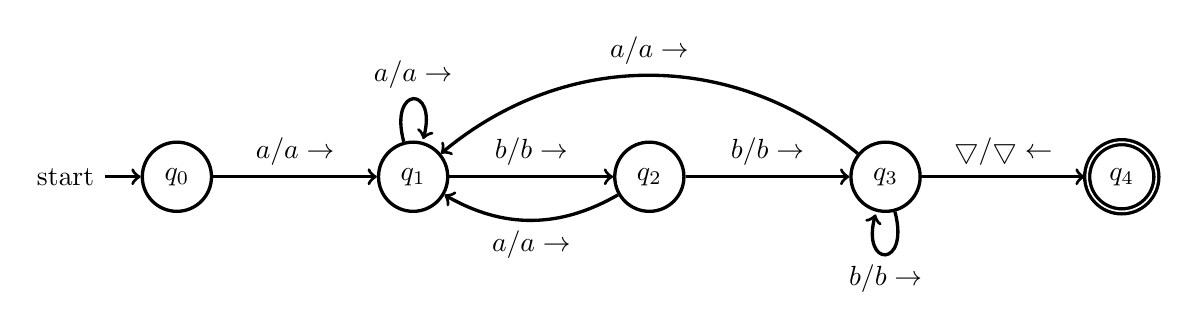
\begin{tikzpicture}[->,node distance=3cm,auto,very thick]

\node[initial,state](q0){$q_0$};
\node[state](q1)[right of=q0]{$q_1$};
\node[state](q2)[right of=q1]{$q_2$};
\node[state](q3)[right of=q2]{$q_3$};
\node[state,accepting](q4)[right of=q3]{$q_4$};

\path(q0)edge node[above]{$a/a\rightarrow$}(q1)
	(q1)edge[loop above] node[above]{$a/a\rightarrow$}()
	(q2)edge[bend left] node[below]{$a/a\rightarrow$}(q1)
	(q2)edge node[above]{$b/b\rightarrow$}(q3)
	(q3)edge node[above]{$\bigtriangledown/\bigtriangledown\leftarrow$}(q4)
	(q3)edge[bend right=1.4cm] node[above]{$a/a\rightarrow$}(q1)
	(q1)edge node[above]{$b/b\rightarrow$}(q2)
	(q3)edge[loop below] node[below]{$b/b\rightarrow$}();

\end{tikzpicture}
\end{center}

\newpage

\noindent\textbf{Zad 1.47.} Wypisz cztery przykładowe łańcuchy opisywane przez wyrażenie \textbf{10+(0+11)$\textbf{0}^*$1}. Czy można skonstruować (deterministyczną) maszynę Turinga, która akceptuje język
\[L=L(\textbf{10+(0+11)$\textbf{0}^*$1})?\]
Jeżeli można, to narysuj diagram przejść i dla zaprojektowanej maszyny wy-konaj dwa obliczenia (wykonaj rysunki taśmy i zapisz konfiguracje).

 Rozwiązanie.
 
\[M=(Q,\Gamma,\Sigma,\delta,q_0,\bigtriangledown,F)=(\{q_0,...,q_8\},\{1,0\},\{1,0,\bigtriangledown\},\delta,q_0,\bigtriangledown,\{q_8\}).\]

\begin{center}
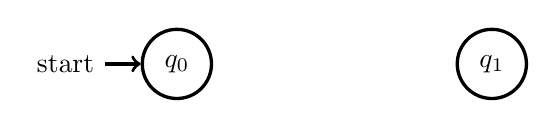
\begin{tikzpicture}[->,node distance=4cm,auto,very thick]

\node[initial,state](q0){$q_0$};
\node[state](q1)[right of=q0]{$q_1$};

\end{tikzpicture}
\end{center}

\end{document}